%!TEX program = xelate
%%%%%%%%%%%%%%%%%%%%%%%%%%%%%%%%%%%%%%%%%
% Modified By Orcuslc, 2016-9-21
% Modified for Assignments
% http://github.com/orcuslc
%
% Wilson Resume/CV
% Structure Specification File
% Version 1.0 (22/1/2015)
%
% This file has been downloaded from:
% http://www.LaTeXTemplates.com
%
% License:
% CC BY-NC-SA 3.0 (http://creativecommons.org/licenses/by-nc-sa/3.0/)
%
%%%%%%%%%%%%%%%%%%%%%%%%%%%%%%%%%%%%%%%%%

%----------------------------------------------------------------------------------------
%	PACKAGES AND OTHER DOCUMENT CONFIGURATIONS
%----------------------------------------------------------------------------------------
\documentclass[10pt]{article}

\usepackage{listings}
\usepackage{xcolor}
\usepackage{amsmath,amsthm,amssymb}
\usepackage{epstopdf}
\usepackage{graphicx}
\usepackage{clrscode3e}

\DeclareGraphicsExtensions{.eps,.ps,.jpg,.bmp}


\usepackage[a4paper, hmargin=25mm, vmargin=30mm, top=20mm]{geometry} % Use A4 paper and set margins

\usepackage{fancyhdr} % Customize the header and footer

\usepackage{lastpage} % Required for calculating the number of pages in the document

\usepackage{hyperref} % Colors for links, text and headings

\setcounter{secnumdepth}{0} % Suppress section numbering

%\usepackage[proportional,scaled=1.064]{erewhon} % Use the Erewhon font
%\usepackage[erewhon,vvarbb,bigdelims]{newtxmath} % Use the Erewhon font
\usepackage[utf8]{inputenc} % Required for inputting international characters
\usepackage[T1]{fontenc} % Output font encoding for international characters

\usepackage{fontspec} % Required for specification of custom fonts
\setmainfont[Path = ./fonts/,
Extension = .otf,
BoldFont = Erewhon-Bold,
ItalicFont = Erewhon-Italic,
BoldItalicFont = Erewhon-BoldItalic,
SmallCapsFeatures = {Letters = SmallCaps}
]{Erewhon-Regular}

\usepackage{color} % Required for custom colors
\definecolor{slateblue}{rgb}{0.17,0.22,0.34}

\usepackage{sectsty} % Allows customization of titles
\sectionfont{\color{slateblue}} % Color section titles

\fancypagestyle{plain}{\fancyhf{}\cfoot{\thepage\ of \pageref{LastPage}}} % Define a custom page style
\pagestyle{plain} % Use the custom page style through the document
\renewcommand{\headrulewidth}{0pt} % Disable the default header rule
\renewcommand{\footrulewidth}{0pt} % Disable the default footer rule

\setlength\parindent{0pt} % Stop paragraph indentation

% Non-indenting itemize
\newenvironment{itemize-noindent}
{\setlength{\leftmargini}{0em}\begin{itemize}}
{\end{itemize}}

% Text width for tabbing environments
\newlength{\smallertextwidth}
\setlength{\smallertextwidth}{\textwidth}
\addtolength{\smallertextwidth}{-2cm}

\newcommand{\sqbullet}{~\vrule height .8ex width .6ex depth -.05ex} % Custom square bullet point 


\newcommand{\tbf}[1]{\textbf{#1}}
\newcommand{\tit}[1]{\textit{#1}}
\newcommand{\mbb}[1]{\mathbb{#1}}
\newcommand{\blue}[1]{\color{blue}{#1}}
\newcommand{\red}[1]{\color{red}{#1}}
\newcommand{\sblue}[1]{\color{slateblue}{#1}}
\newcommand{\n}{\\[5pt]}
\newcommand{\tr}{^\top}
\newcommand{\vt}[1]{
\Vert #1 \Vert
}
\newcommand{\bra}[5]{
#1=\left\{
\begin{aligned}
#2 ,&\quad #4 \\
#3 ,&\quad #5
\end{aligned}
\right.
}

\renewcommand{\title}[2] {
{\Huge{\color{slateblue}\textbf{#1}}}
\hfill
\LARGE{\color{slateblue}\textbf{#2}} \\[10pt]
\large{\color{slateblue}\textbf{Chuan Lu, 13300180056, chuanlu13@fudan.edu.cn}} \\[1mm]
\rule{\textwidth}{0.5mm}
}

\newcommand{\problem}[2] {
\vspace{20pt}
\LARGE{\color{slateblue}\textbf{Problem #1.}}
\vspace{2mm}
#2 \\[10pt]
}

\renewcommand{\proof}[2] {
\large{\color{slateblue}\textit{\textbf{#1.}}}
#2 \qed \\[3mm]
}

\newcommand{\solution}[2] {
\large{\color{slateblue}\textit{\textbf{#1.}}}
#2 \\[3mm]
}


\newcommand{\algorithm}[2] {
\begin{codebox}
\Procname{$\proc{Algorithm #1}$}
#2
\end{codebox}
}

\newcommand{\refgroup}[1] {
\LARGE{\color{slateblue}\textbf{Reference}} 
\begin{tabbing}
\hspace{5mm} \= \kill
#1
\end{tabbing}
}

\newcommand{\reference}[1] {
\sqbullet \ \  \large{#1} \\
}
% \newcommand{\solution}[2] {
% \LARGE{\color{slateblue}\textit{#1}}
% \ #2 \qed
% }

% \newenvironment{problem}[2][Problem]{\begin{trivlist}
% \item[\hskip \labelsep {\bfseries #1}\hskip \labelsep {\bfseries #2.}]}{\end{trivlist}}
\usepackage{epstopdf}
\usepackage{graphics}
\usepackage{subfig}
\usepackage{listings}
\lstset{
  breaklines=true,
  xleftmargin=25pt,
  xrightmargin=25pt,
  aboveskip=0pt,
  belowskip=10pt,
  basicstyle=\ttfamily,
  showstringspaces=false,
  frame=ltrb,
  tabsize=4,
  numbers=left,
  numberstyle=\small,
  numbersep=8pt,
  morekeywords={*, factorial, sum, erlang},
  keywordstyle=\color{blue!70}, commentstyle=\color{red!50!green!50!blue!50},
}
\DeclareGraphicsExtensions{.eps,.ps,.jpg,.bmp}

\begin{document}

\title{Numerical Analysis \\ Assignment 9}
\date{\today}
\author{Chuan Lu}

\maketitle

\problem{1}{Problem 4.1, Page 239.}
\solution{Solution}{
When $n = 4$,
$$
\begin{aligned}
p_4(x) &= \sum_{k=0}^{4}C_{4}^kf(\frac{k}{4})x^k(1-x)^{4-k} = f(0)(1-x)^4 + 4f(\frac{1}{4})x(1-x)^3 + 6f(\frac{1}{2})x^2(1-x)^2+4f(\frac{3}{4})x^3(1-x) + f(1)x^4 \\
&= (6-4\sqrt{2})x^4 + 8\sqrt{2}x^3 - (12+6\sqrt{2})x^2 +2\sqrt{2}x+6 \\
&= (6-4\sqrt{2})(x-\frac{1}{2})^4-3(x-\frac{1}{2})^2+3+\frac{\sqrt{2}}{4}
\end{aligned}
$$
And the fourth degree Taylor polynomial expanded about $\frac{1}{2}$ is
$$
\begin{aligned}
q_4(x) &= f(\frac{1}{2}) + f'(\frac{1}{2})(x-\frac{1}{2}) + \frac{1}{2}f''(\frac{1}{2})(x-\frac{1}{2})^2+\frac{1}{6}f^{(3)}(\frac{1}{2})(x-\frac{1}{2})^3 + \frac{1}{24}f^{(4)}(\frac{1}{2})(x-\frac{1}{2})^4 \\ 
&= 1-\frac{1}{2}\pi^2(x-\frac{1}{2})^2+\frac{1}{24}\pi^4(x-\frac{1}{2})^4
\end{aligned}
$$
}
When $x \to\frac{1}{2}$, $q_4(x) \to 1 = f(\frac{1}{2})$, while $p_4(x) \to 3+\frac{\sqrt{2}}{4}$. Thus Bernstein polynomials are poor approximations.

\problem{2}{Problem 4.5, Page 240}
\solution{Solution}{
First we have 
$$
R(0) = a, ~R'(x) = \frac{b-ac}{(1+cx)^2}, ~R'(0) = b-ac,
$$
$$
R''(x) = -2c(b-ac)(1+cx)^{-3}, ~R''(0) = -2c(b-ac).
$$
This kind of approximation does not necessarily exists. For example, if we choose $f$, s.t. $f'(x) = xe^{x}$. Then $f''(x) = (1+x)e^{x}$, and $f'(x) = 0, f''(x) = 1$. But since $R''(0) = -2cR'(0) = 0$, it makes a contradiction.
}

\problem{3}{Problem 4.6, Page 240}
\solution{Solution}{
$$R(0) = a = f(0) = 1,$$	
$$
R'(0) = b-ac = f'(0) = 1,
$$
$$
R''(0) = -2c(b-ac) = f''(0) = 1.
$$
Then $a = 1, b = \frac{1}{2}, c = -\frac{1}{2}$. Thus
$$
R(x) = \frac{1+\frac{1}{2}x}{1-\frac{1}{2}x}.
$$
And
$$
f(x) - R(x) = e^x-\frac{e^{\frac{1}{2}x}-\frac{1}{2}f''(\xi)(\frac{1}{2}x)^2}{e^{-\frac{1}{2}x}-\frac{1}{2}f''(\eta)(-\frac{1}{2}x)^2} = \frac{\frac{1}{8}(e^\eta+e^\xi)x^2}{e^{-\frac{1}{2}x}-\frac{1}{8}e^{\eta}x^2} = \frac{(e^\eta+e^\xi)x^2}{8-4x},
$$
Then
$$
\max_{x\in[-1, 1]}|f-R| \le \frac{e}{2}.
$$
Since 
$$
|f-p_2| = |\frac{1}{6}e^\eta x^3| \le \frac{e}{6},
$$
So the supremum of error of Pade approximation could be larger than Taylor polynomial.
}

\problem{4}{Problem 4.10, Page 241}
\solution{(a)}{
The linear Taylor polynomial to $f = \ln(x)$ expanding about $\frac{3}{2}$ is
$$
p_1(x) = \frac{3}{2} + \frac{2}{3}(x-\frac{3}{2}) = \frac{2}{3}x+\frac{1}{2}.
$$
The error of is as follows, the left is error graph for (a) and the right is for (b).
}
\solution{(b)}{
The linear minimax approximation to $f$ is 
$$
p_2(x) = ax+b.
$$
Then there exists $x_0$, s.t. 
$$
\ln(1) - (a+b) = \ln(2) - (2a+b) = -(\ln(x_0)-(ax_0+b)) = \rho. 
$$
and
$$
(\ln(x)-(ax+b))'|_{x_0} = 0
$$
Then we have
$$
a = \ln(2), ~x_0 = \frac{1}{\ln(2)}, b = \frac{1}{2}(\ln(\frac{1}{2}\ln(2))+1),
$$
thus
$$
p_2(x) = \ln(2)x+\frac{1}{2}(\ln(\frac{1}{2}\ln(2))+1)
$$
}
\begin{figure}
\begin{minipage}{0.5\textwidth}
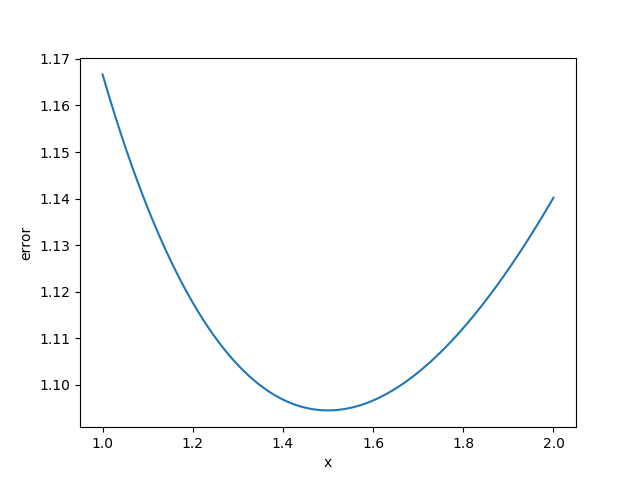
\includegraphics[width = \textwidth]{prob10a.png}
\end{minipage}
\begin{minipage}{0.5\textwidth}
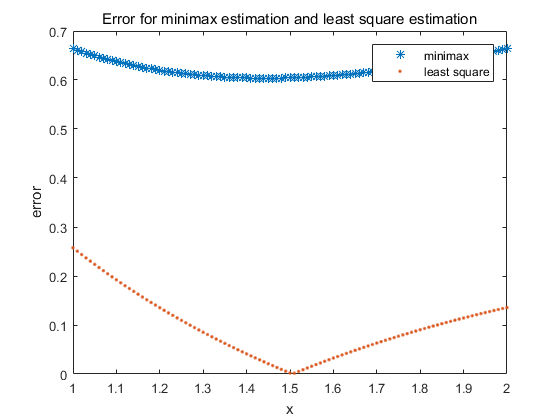
\includegraphics[width = \textwidth]{prob10b.png}
\end{minipage}
\end{figure}

\problem{5}{Problem 4.12, Page 241}
\solution{Solution}{
The linear least square approximation to $f$ is 
$$
q(x) = ax+b.
$$
Then
$$
E = \int_{1}^2 (\ln(x)-ax-b)^2 dx,
$$
and
$$
\frac{\partial E}{\partial a} = \int_{1}^{2} (-2x)(\ln(x)-ax-b)dx = 0,
$$
$$
\frac{\partial E}{\partial b} = \int_{1}^{2} (-2)(\ln(x)-ax-b)dx = 0.
$$
Then 
$$
\left\{
\begin{aligned}
&\frac{3}{2}a+\frac{3}{2}b = 2\ln(2)-1 \\
&\frac{14}{3}a+3b = 4\ln(2)-2
\end{aligned}
\right.
$$
solving this equations, we get 
$$
a = 0.3, ~b = \frac{4}{3}\ln(2)-\frac{29}{30}.
$$
The error graph is showed in (b) of Problem 4.
}

\end{document}